\chapter{Introduction and Motivation}\label{ch:intro}


Lung cancer is one of the most common {cancers} in the world. It is the prevalent cancer type both in incidence and mortality in men and third in incidence and second in mortality, after breast cancer, in women\cite{WCR2014}. Death due to lung cancer surpass 1.5 million a year(see figure \ref{fig:world} for incidence), having around 10\% of five year survival rate in developed countries, and much lower in developing countries\cite{CRUK2014}. One in fourteen people has a lifetime risk of developing lung cancer\cite{Harrisons2012}, on average between men and women. The high incidence and mortality rates has lead to a high research throughput in mutidiciplinary fields, in order advance further the detection and treatment techniques of the disease, resulting in an output of over 23.000 lung cancer related research articles in reputable journals in the last 10 years\cite{Nature2015}. At the same time, the  actual lung cancer treatment has been transformed from non-existent in the 70s to being available worldwide\cite{Comis2003}.


\begin{figure}[ht]
\begin{center}
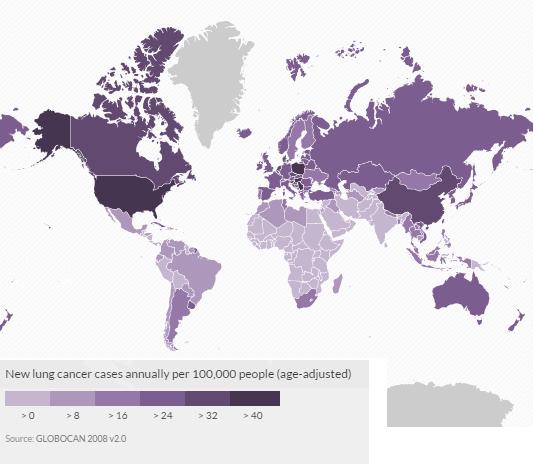
\includegraphics[width=0.65\columnwidth]{StateOfArt/worldmap.png}
\caption[Lung cancer incidence in the world]{Lung cancer incidence per country, age adjusted data. Map and data from {GLOBOCAN}\cite{GLOBOCAN2010}.}
%IARC has proprietary rights to the materials on the Website. Publications/data made available by IARC/WHO enjoy copyright protection in accordance with the provisions of Protocol 2 of the Universal Copyright Convention. All rights are reserved. Materials (fact sheets, maps, estimates or data) may be used "as is" for research, educational or other non-commercial purposes, but the corresponding reference must be cited in all cases.
\label{fig:world}
\end{center}
\end{figure}

Lung cancer treatment, while diverse between types of cancer, can be classified in four main types: chemotherapy, lobectomy or pneumoctomy, radiotherapy (RT) and palliative care. Generally, in early stages of small cell lung cancer the common treatment would consist in chemotherapy with radiotherapy, usually followed by brain radiotherapy, as there is a chance of metastasis in the brain. In the unlikely chance that the tumour is detected at a very early stage and has not spread to the lymph nodes, a lobectomy may be performed, removing part of the lung. Usually this is followed by radiotherapy and chemotherapy to make sure the tumour is completely removed.
In the case of non-small cell lung cancer, in the first stages the patient may undergo a lobectomy or a pneumoctomy (removal of the whole lung). Generally radiotherapy and chemotherapy (less likely) are added to the treatment in this case too. In the last stages of the lung cancer, usually the treatment is palliative care i.e. treatments to reduce the symptoms and relieve pain\cite{CRUK2014b}.

In practically all stages of different lung cancer treatments, radiotherapy is extensively used as above half of the treated patients do undergo the procedure\cite{Cancerorg}, with around 120,000 patients are treated with radiotherapy in the UK every year. Radiotherapy is a non-invasive technique that aims to destroy malignant cells using ionizing radiation, generally using photons. This is possible because high energy photons (X-rays) ionize the atoms that are part of the DNA chain, damaging it thus causing cellular death. In photon therapy, this happens due to the ionization of the water in the cells, that forms free radicals, such as hydroxyl radicals, destroying the DNA of the cells. Conventional photon RT is widely used around the world.

However, a different type of radiation therapy exists, particle therapy or hadron therapy, that uses charged particles instead of photons, by accelerating them with circular particle accelerators. These particles (protons and heavy ions)  penetrate the tissue with minimal interaction and release almost all the energy before stopping. Figure \ref{fig:bragg} shows the energy deposition (dose) plotted versus the penetration of the energy beam in tissue. The energy burst that hadrons show is referred to as the Bragg peak, after its discoverer William Henry Bragg. The Bragg peak allows for a radiation therapy where a larger amount of healthy tissue can be spared, while delivering highly spatially accurate doses to only the tumour areas. While the growth of hadron therapy has been slow in the past due to its cost, it is now being accelerated thanks to international collaboration projects such as ENLIGHT\cite{dosanjhparticle}, with 100 centres estimated by 2020 around the globe, 30 of them in Europe, 3 of them being already in their final stages in construction in the UK.

\begin{figure}[ht]
\begin{center}
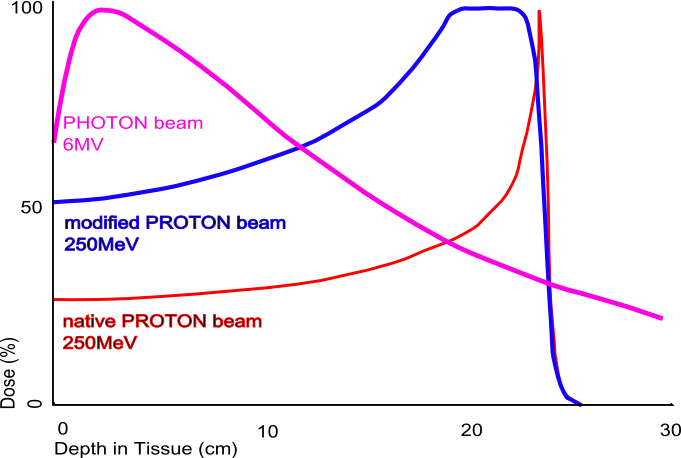
\includegraphics[width=0.6\columnwidth]{Introduction/BraggPeak.png}
\caption[Bragg peak]{ Depth-dose curves for photons (X rays) and protons (monoenergetic: red, polyenergetic:blue, indicating the different dose deposition behaviour of photons and charged particles when traversing matter. The ``spread-out Bragg peak'' can be tailored to provide a highly conformal dose deposit to the tumour volume, thus largely sparing surrounding healthy tissue from unwanted dose deposition. The proposal of  exploiting the favourable properties of heavy charged particles for cancer treatment was first proposed by Wilson\cite{wilson1946radiological}.}
%GNU license, wikipedia
\label{fig:bragg}
\end{center}
\end{figure}


RT treatment is nowadays generally guided by imaging systems during treatment planning (image guided radiation therapy, IGRT). Imaging systems, such as computed tomography (CT) and magnetic resonance imaging (MRI) are used to carefully tune the X-ray beam to focus in the specific location and shape of the tumour, and monitor the effects during the whole treatment period. Tumours not only are very different between patients, but also change considerably during treatment, so does the patient due to the physical toll of cancer treatment. This means that the tumour does change both shape and location and that, if these changes are not known, healthy tissue could be damaged and cancerous tissue spared. Generally, patients will be imaged before each treatment,  one of the most common systems for imaging being cone beam computed tomography (CBCT). CBCT takes several minutes to scan a patient due to mechanical safety limitations. As one can foresee, this is an important limiting factor for tumours that move, such as the liver and the lung ones, as the motion during acquisition can generate heavy artefacts around the moving parts in image reconstruction. This moving effect is also an important factor to be taken into account in hadron therapy, as having a moving tumour means a high chance of missing the treatment target. Providing accurate imaging not only in space, but also in time (4D imaging) is a key factor in treatment planning, \textcolor{blue}{and} thus in cancer treatment. Figure \ref{fig:motionblurr} shows the motion artefacts common in CBCT.

Interestingly, a motion compensation method for when objects are moving during {acquisition} was proposed by Hancock \textit{et al}\cite{pst1}\cite{pst2}\cite{pstweb} for monitoring the phase space of high energy particle bunches in particle accelerators at CERN. Phase space tomography is a hybrid algorithm that combines particle tracking in a computer model of a synchrotron with iterative reconstruction algorithms to reconstruct an image of the population of a bunch of particles circulating in the accelerator. The particle motion involves \tb{a complex non-uniform rotation across the phase space} and is non-cyclic, but a 1D projection of the distribution can be completely acquired as a single snapshot \tb{on} one turn of the machine. By tracking test particles to gain a knowledge of how the geometry of the 2D image plane (longitudinal phase space) deforms, the information in all the discrete time slices acquired over many turns can be translated back to the same instant and tomographically combined in a single image.  Exploring the feasibility of using this tomographic motion compensation technique in medical applications is the objective of this thesis.

\begin{figure}

\begin{center} 
\subfigure[]{ 
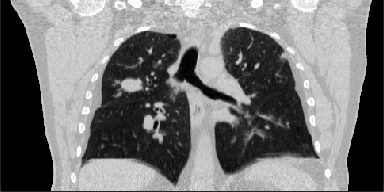
\includegraphics[width=0.4\linewidth]{Introduction/static.png} 
}
\subfigure[]{ 
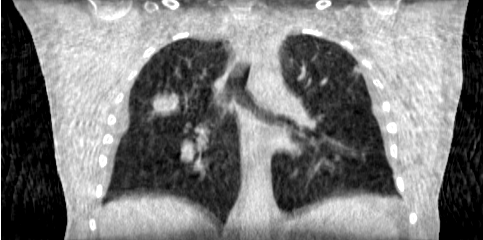
\includegraphics[width=0.4\linewidth]{Introduction/motionblur.png} 
}
 
\caption[Motion blurr in lung CBCT]{\label{fig:motionblurr}(a) Static CT image of a patient (from a 4D-CT dataset) (b) motion artefacts when reconstructed using data acquired from various breathing periods (simulated). The dataset is the POPI model\cite{popi-modelweb}.}
\end{center} 
\end{figure}


%% BLURRED IMAGE OF TUMOUR

\section{Aim of the thesis}

CBCT and computed tomography (CT) in general image reconstruction problem is a complex mathematical and computational challenge, even for just 3D spatial reconstruction, without the additional problem of motion. Mathematically CT reconstruction is an ill-posed problem and generally the volume to reconstruct is considerably larger than the data obtained, making the problem underdetermined. Often, an analytic approximated solution for the  mathematical problem is used, however this solution is considerably sensitive to noise and low amounts of data. As opposed to the analytic approximated solution, algebraic equation solving methods can be used. These generally lead to more robust solutions, especially with noisy and undersampled data. However, they require increased computational times, making them harder to introduce to clinical applications. There are two main research problems tackled in this work:

\begin{itemize}
\item Firstly, this thesis explores the image reconstruction problem, with a focus on implementing accurate iterative algorithms, and accelerating them as much as possible, using GPU technology. The results from this part of the thesis are applicable to any CT application, from the medical one, to industrial or research cases. The work here explores a variety of algorithms for CT reconstruction, with both mathematical and computational focus.
\item Secondly, the thesis concentrates on translating the motion compensation methods to the medical CBCT, focusing on \tb{lung} IGRT applications, focusing also on the computational side of the method, as well as its robustness.
\end{itemize}

All the research presented here has been made public as part of the TIGRE Toolbox\cite{TIGRE} and can be found in a GitHub repository\cite{TIGREweb} for both MATLAB and Python. 

\section{Thesis organization}

The chapters of this thesis try to be a self contained document. However, it can be separated into two main topics: GPU-based CT reconstruction (Chapters 3, 4 and 5) and motion compensation methods for IGRT (Chapters 2, 6 and 7). \tb{Chapter 8 concludes the thesis and proposes future work.} The contents of each chapter are summarized as follows:

\subsubsection{Chapter 2: Image Guided Radiation Therapy and Computed Tomography}


\begin{wrapfigure}{L}{0.35\textwidth}
\centering
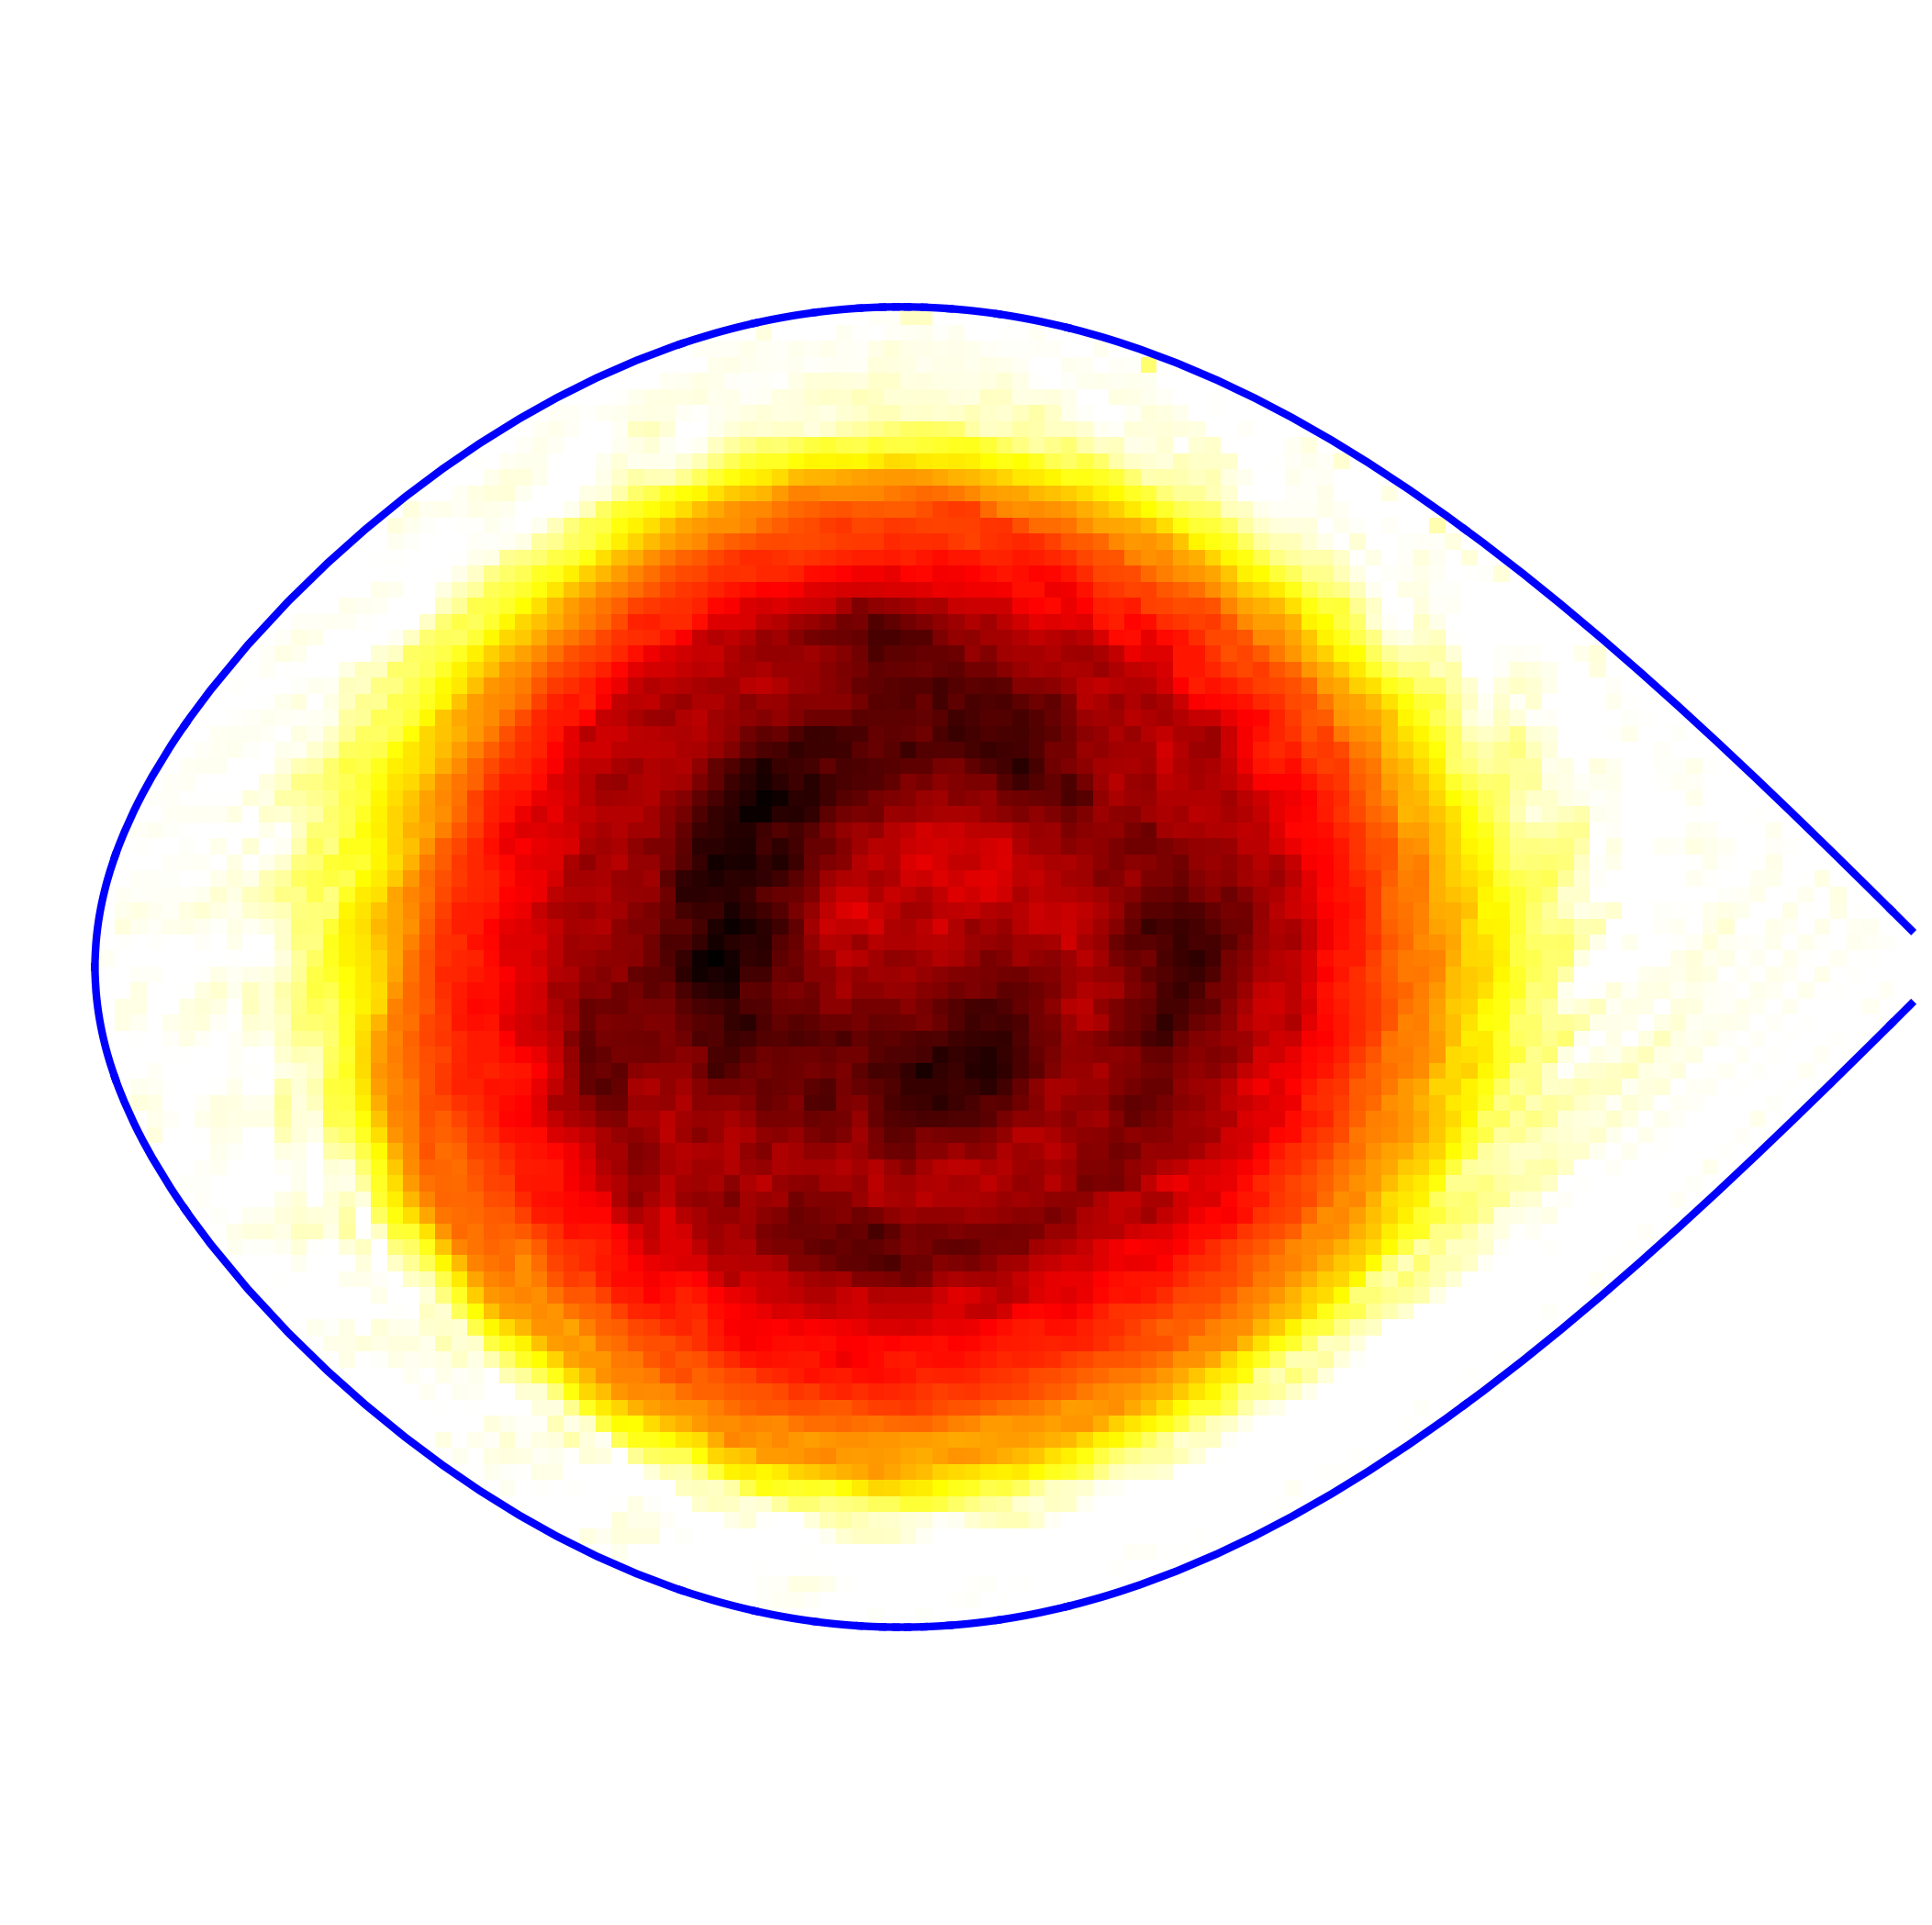
\includegraphics[width=0.32\textwidth]{StateOfArt/pst.png}
\end{wrapfigure}

An introduction to IGRT, focusing on imaging and the challenges in providing quality imaging for radiation treatment for both photon and hadron radiation therapy. As CBCT is one of the most widely used imaging systems for IGRT, a further study into the innovations of CBCT is presented, focusing after on the research available for dealing with non-rigid motion, such as respiratory motion. This exhaustive research shows that the vast majority of motion compensation algorithm are based on binning the data according to breathing phase and reconstructing an image for each bin, while very few publications exist with a similar concept for motion compensation as the phase space tomography, with no computational focus. Finally, there is a brief description of the wider uses of CT in general, from research to industry.

\vspace{40pt}
\subsubsection{Chapter 3: The Image Reconstruction Problem}

\begin{wrapfigure}{L}{0.35\textwidth}
\centering
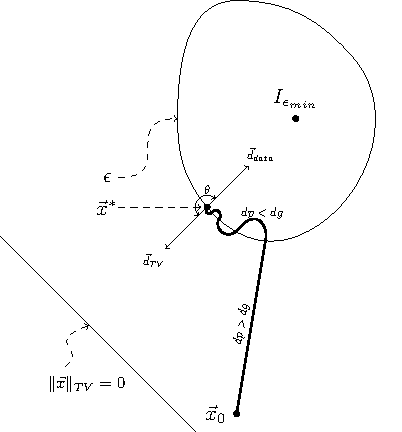
\includegraphics[width=0.32\textwidth]{RecAlgorithms/POCS.pdf}
\end{wrapfigure}

CBCT image reconstruction is an ill-posed problem, \tb{where even if solution may exists a stable numerical solution for it is not feasible\cite{Finch}}. Substandard conditions on the data acquisition process (such as noise, or geometric errors) and limited data can have a severe influence on the quality of the image reconstructed, especially using the Feldkamp Davis and Kress (FDK) method that approximates the analytic solution. However FDK is the most commonly used algorithm across the field. The reconstruction problem can however be described as an algebraic minimization problem, and iterative solvers can be used for minimization. This chapter describes briefly FDK and continues to showcase the mathematics of a variety of different iterative solvers for CBCT, such as SART and similar methods, Krylov subspace methods and a variety of total variation regularized iterative methods.
\FloatBarrier
\subsubsection{Chapter 4: GPU methods in tomography}



\begin{wrapfigure}{L}{0.35\textwidth}
\centering
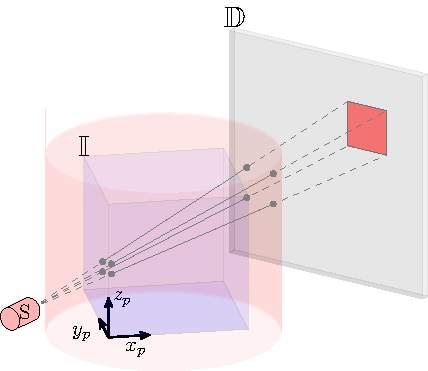
\includegraphics[width=0.32\textwidth]{GPUmethods/projcoord-figure0.pdf}
\end{wrapfigure}

CBCT reconstruction is a computationally very expensive problem. Iterative algorithms only enhance this problem, as they require sometimes hundreds of iterations, each of them being more costly than a single FDK solution. This chapter shows how GPU computing can accelerate the image reconstruction by tailoring very fast algorithms to GPU computational structure. It describes how the projection and backprojection operators (the basic building blocks of CT reconstruction) are implemented to reach state of the art speeds using different X-ray approximation methods. Finally, after showing how these have been used together with the mathematics of Chapter 3 to build the TIGRE Toolbox, an easy to use, free, flexible, modular and fast MATLAB and Python with CUDA toolbox is presented. 
\FloatBarrier


\newpage
\subsubsection{Chapter 5: Experiments and applications}

\begin{wrapfigure}{L}{0.35\textwidth}
\centering
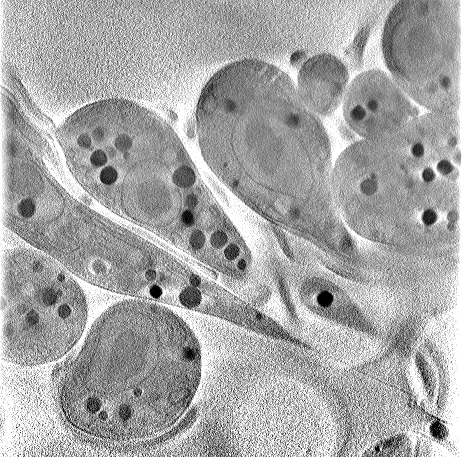
\includegraphics[width=0.27\textwidth]{Applications/thumnail.png}
\end{wrapfigure}

This chapter explores some behaviour of iterative algorithms implemented on GPUs and shows how some of the algorithms behave with different datasets. Firstly some numerical experiments are performed for digital phantoms, analysing the effect of angle ordering on SART-type algorithms, hyperparameter reduction methods and observing the behaviour of the different TV algorithms included in TIGRE. Then some real datasets are reconstructed using a variety of the algorithms presented in previous chapters, from medicine (a head phantom from the Christie Hospital), micro-tomography (the Sofia-beads dataset) and synchrotron tomography (some cryo soft X-ray tomograms). One of these last datasets is then segmented using the {SuRVoS} workbench to highlight the differences.


\FloatBarrier
\subsubsection{Chapter 6: motion compensation modelling}

\begin{wrapfigure}{l}{0.35\textwidth}
\centering
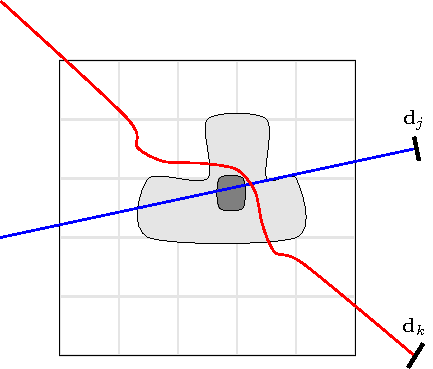
\includegraphics[width=0.32\textwidth]{MotionCorrection/diagrammotion1.pdf}
\end{wrapfigure}

Using the theory from phase space tomography at CERN, this chapters proposes a motion compensation algorithm for when the motion is approximately known. By modelling the X-rays as warped paths instead of straight lines on the GPU. The GPU implementation is described and two experiments are presented, one with synthetic data and deformation  vector fields, and another one using a 4D-CT dataset. Results show that when the motion is perfectly known the method performs equally well to a reconstruction without motion and that the method can give better information about the tumour using the same amount of projections as a CBCT image. As the method relies on modelling the motion in the basic building blocks of CT reconstruction, it can be used in any existing iterative algorithm.



\newpage
\FloatBarrier
\subsubsection{Chapter 7: Numerical Study of Motion Compensation}

\begin{wrapfigure}{L}{0.35\textwidth}
\centering
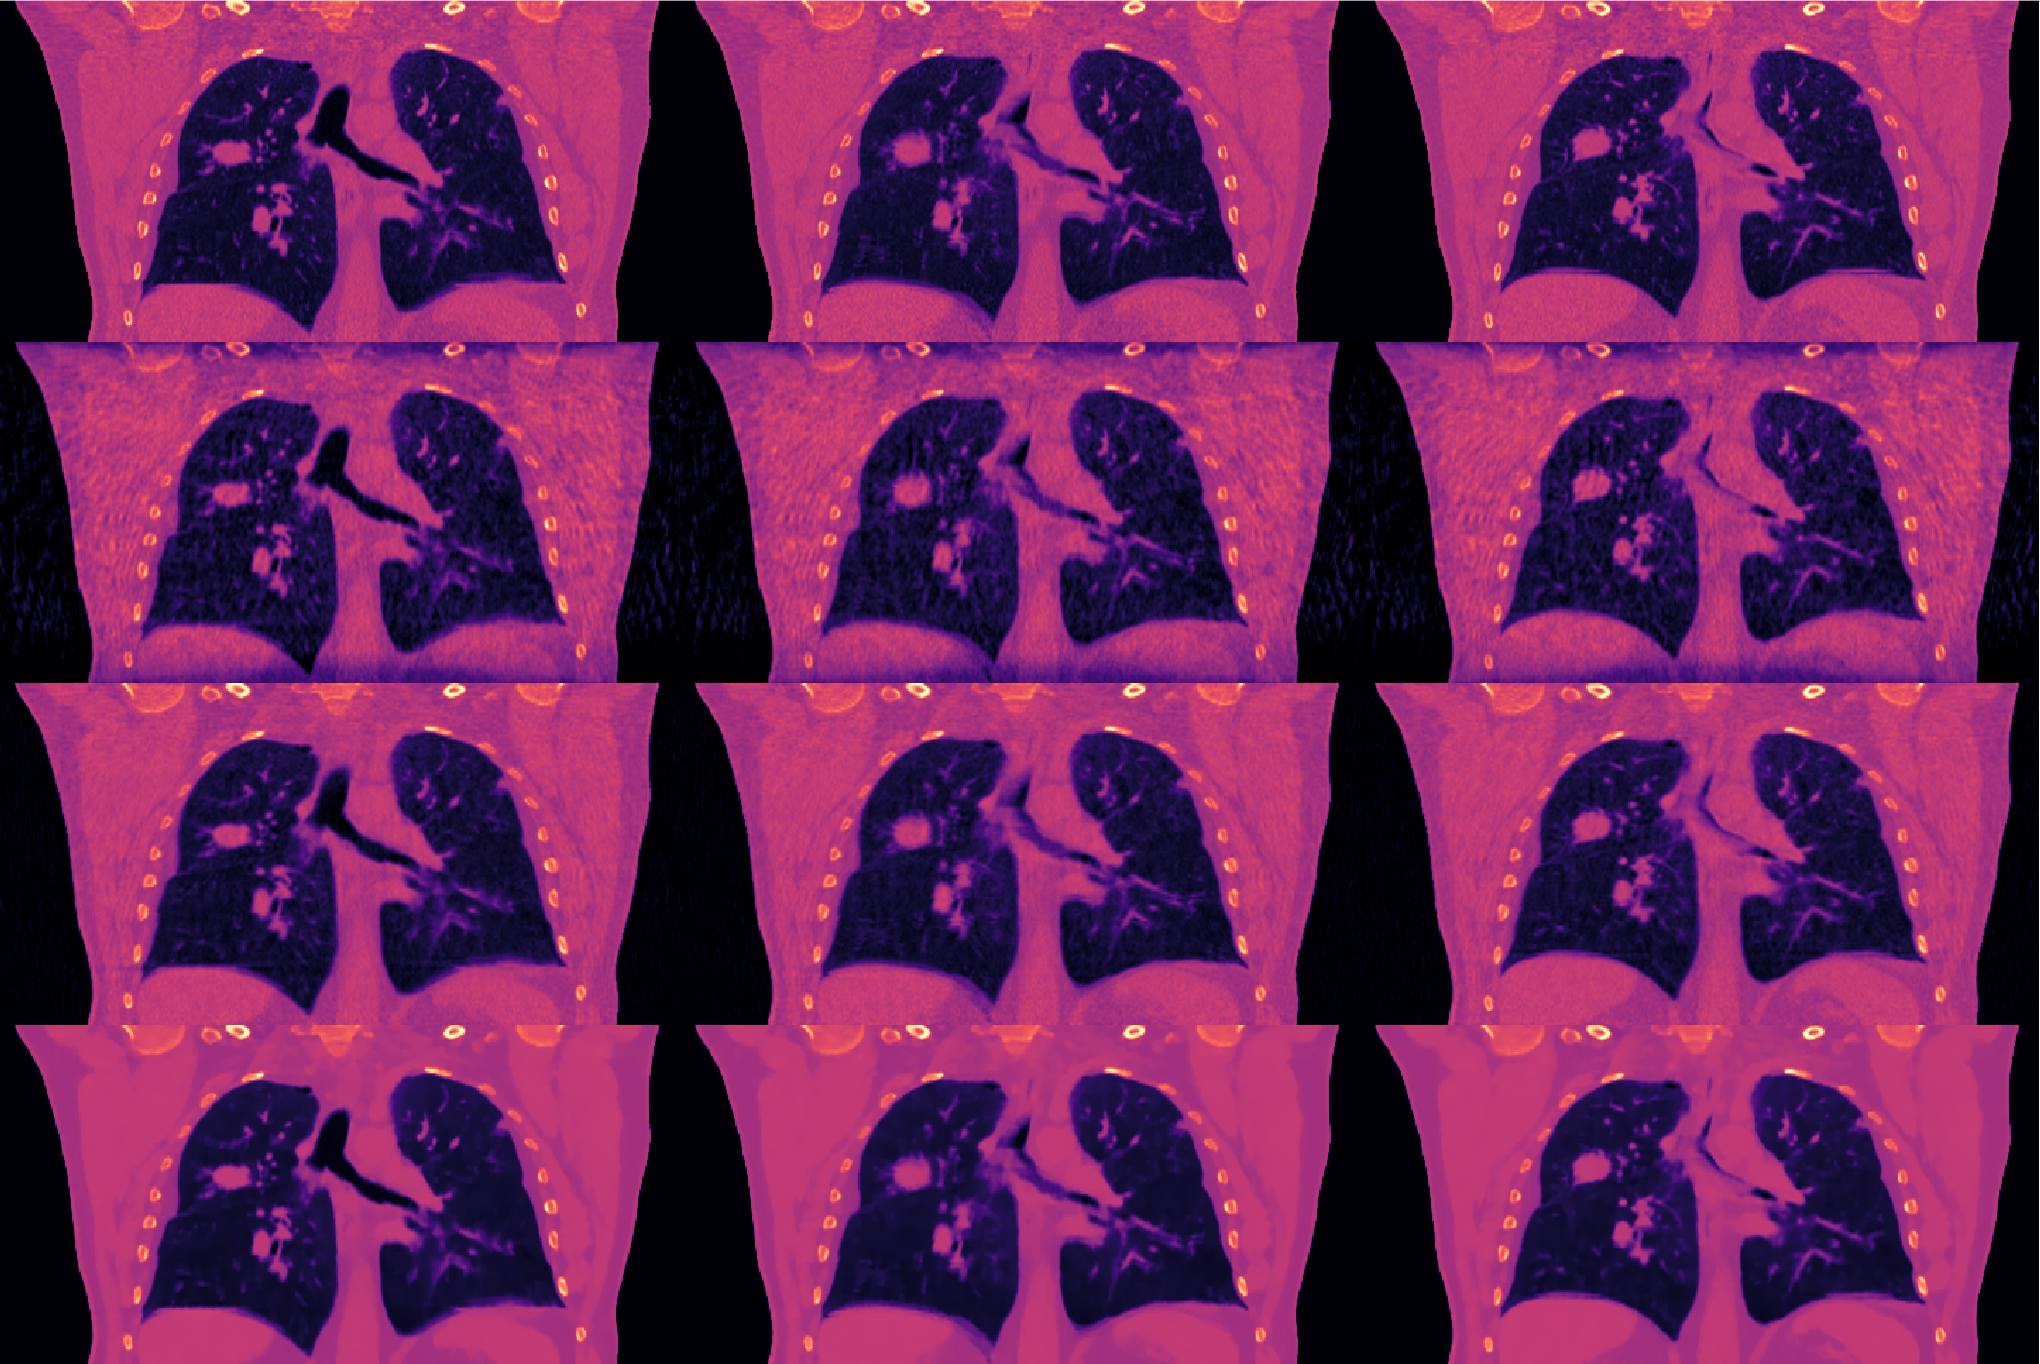
\includegraphics[width=0.32\textwidth]{accuracyMC/4DCBCT3stage.png}
\end{wrapfigure}
The previous chapter described a method for motion compensation. This chapter focuses on numerically testing the limits of the method, as obtaining perfect motion information is an almost impossible task in medical applications. The chapter shows that the performance of the method is very similar (with marginally bigger error) than 4D-CBCT, with an order of magnitude less projections, thus less radiation to the patient. Tests against the most common numerical errors in medical applications are performed: very low resolution motion information, errors in the binning process of projections (thus in the motion information) and the case where only the motion of the tumour is known. In all cases, the motion compensation method has errors of less than a voxel in tumour location, and very small mismatch in the volume selection of the tumour.




\FloatBarrier


\section{Publications and contributions}

The work on this thesis was been published either as open source software or publications in conferences and peer reviewed journals. The following publications directly relate to the content of this thesis:

\begin{itemize}
\item ``GPU based iterative CBCT for prospective motion compensated algorithm for radiation therapy''\cite{biguri2016gpu}. Short paper based on the presentation at the conference ICTR-PSE 2016. \tb{The author of this thesis contribution has been the writing up of the entire toolbox presented. The other authors supported this work with contribution on the context, importance and presentation of the work.}
\item ``TIGRE: A MATLAB-GPU toolbox for CBCT image reconstruction''\cite{TIGRE}. Journal article condensing the research in Chapter 3, Chapter 4 and Chapter 5. \tb{Similarly as the previous article, most of the article and code has been written by the author of this thesis. The other authors supported this work with contribution on the context, importance and presentation of the work.}
\item  ``A General Method for Motion Compensation in X-ray Computed Tomography''\cite{biguri2017general}. Journal article on Chapter 6. \tb{The original idea came from S. Hancock, A. Biguri translated that knowledge into a practical algorithm with GPUs for the medical case, due to the difference in scale an physics of the problems. M. Dosanjh contributed with the biomedical knowledge of the relevance of the methods for IGRT and M. Soleimani with supervision on the project and mathematics.}
\end{itemize}

This work has been also presented in various conferences and meetings, via posters or presentation talks. Posters have been presented at ToScA 2016 with the title ``TIGRE: Tomographic Iterative GPU-based Reconstruction toolbox''\cite{biguri_ander_2016_159016}, in the ENLIGHT 2016 meeting titled ``Motion correction in X-ray tomography using a priori known deformation vector fields and iterative reconstruction methods''\cite{biguri2016motion} and in BIGART 2017 titled ``Improvement of image quality in 4D-CBCT respiratory correlated and motion-compensated reconstruction using iterative algorithms and GPU acceleration''\cite{biguri2017motion}. The work has also been presented in various talks and seminars. Finally, a Medical Physics Web article by Tami Freeman is available for wider audiences at \href{http://medicalphysicsweb.org/cws/article/research/66343}{http://medicalphysicsweb.org/cws/article/research/66343}.

The TIGRE Toolbox and specifically some of the total variation based image recosntruction code has been also used in the article ``Parameter selection in limited data cone-beam CT reconstruction using edge-preserving total variation algorithms'' by Lohvithee \textit{et al}\cite{Vee}.

\subsubsection{Other publications}

During the course of the PhD, mainly in the early stages, other work was published focused on dual modality electrical impedance tomography (EIT) CBCT, as some initial work explored the use of EIT for real time tumour tracking. That work is not presented in this thesis, but has been published in a few items. The work is summarized in a peer reviewed journal article ``Tracking boundary movement and exterior shape modelling in lung EIT imaging''\cite{biguri2015tracking}, and extended in peer-reviewed conference articles for the EIT 2015 meeting in the works titled ``Statistical and deterministic approaches for electrode movement in lung EIT''\cite{biguri2015statistical} and ``4D FEM models of the human thorax''\cite{biguri20154d}. Initial work in this field was also presented as a poster in the ENLIGHT 2014 meeting titled ``Dual modality EIT-CBCT for lung radiation therapy''\cite{biguri2015dual} and in AIP 2015 as ``Electrode movement due to breathing in lung EIT imaging''\cite{biguri2015electrode}.





